\documentclass[../../main.tex]{subfiles}

\begin{document}

\section{Overview}

This section contains a formal model describing the core parts of the system. The model was defined using \href{https://alloytools.org/}{Alloy}, an open source language and analyzer for software modelling. In particular, customers' line up, store access and store exit events are described.

The following additional assumptions have been added to the model for the sake of simplification, without significant loss of generality:
\begin{itemize}
  \item Time is quantized in time slots; the duration of the time slots is unspecified, thus it would be possible to shrink indefinitely the length of time slots to achieve a very fine level of precision;
  \item Customers leave the store within the time slot limits they requested during the line up request; this is a strong assumption that, however, can be mitigated by the system using the statistical data of the past visits of a customer to provide accurate estimations of the leaving time. In particular, during a line up request, the system could lookup the mean amount of time the customer spent in the store more than they were allowed in the past visits, and add it to the following line up requests.
\end{itemize}

The formal model shows that the system described in the present document:
\begin{itemize}
  \item is consistent with respect to the management of line up requests (i.e., it only accepts a line up request and emits the associated receipt if the requested store does not exceed the maximum number of customers allowed);
  \item is consistent with respect to the access to the store (i.e., it only allows a customer to enter the store if they have a valid line up receipt, they are using it for the first time to access the store and they are entering the store during the assigned time slot);
  \item is consistent with respect to the end of the visit to a store (i.e., it tracks the actual time slots the customer spent in the store);
  \item ensures that no more people than allowed are present inside each store.
\end{itemize}

\section{Alloy model}

\subsection{Source code}

\begin{lstlisting}[language=alloy]
  // Signatures

  sig Customer {
  }
  
  sig Receipt {
    receipt_customer: Customer,
    receipt_startSlot: TimeSlot,
    receipt_store: Store,
    receipt_timeSlots: some TimeSlot
  } {
    receipt_startSlot in receipt_timeSlots
  }
  
  sig Store {
    store_maxCustomersPerSlot: one Int
  } {
    store_maxCustomersPerSlot > 0
  }
  
  sig TimeSlot {
    timeSlot_previous: lone TimeSlot
  }
  
  one sig TIME_SLOT_ZERO extends TimeSlot {}
  one sig TIME_SLOT_CURR extends TimeSlot {}
  one sig TIME_SLOT_MAX extends TimeSlot {}
  
  sig Visit {
    visit_endSlot: lone TimeSlot,
    visit_receipt: Receipt,
    visit_startSlot: TimeSlot,
    visit_store: Store,
    visit_timeSlots: some TimeSlot
  } {
    visit_startSlot in visit_timeSlots and
    visit_endSlot in visit_timeSlots and
    visit_store = visit_receipt.receipt_store
  }
  
  // Utility functions
  
  fun previousTimeSlots [t: TimeSlot] : set TimeSlot {
    t.timeSlot_previous.(*timeSlot_previous)
  }
  
  fun followingTimeSlots [t: TimeSlot] : set TimeSlot {
    timeSlot_previous.t.*(~timeSlot_previous)
  }
  
  fun receiptsForStoreContainingTimeSlot [s: Store, t: TimeSlot] : set Receipt {
    receipt_timeSlots.t <: receipt_store.s
  }
  
  fun visitsInStoreDuringTimeSlot [s: Store, t: TimeSlot] : set Visit {
    visit_timeSlots.t <: visit_store.s
  }
  
  // Constraints on signatures
  
  // Time slots allowed in a receipt are contiguous, and all after the start time slot
  fact {
    all r: Receipt, t: TimeSlot |
      t in r.receipt_timeSlots implies
        (t in r.receipt_startSlot or t.timeSlot_previous in r.receipt_timeSlots) and
        t not in r.receipt_startSlot.previousTimeSlots
  }
  
  // Time slots used for a visit are contiguous, and all after the start time slot and before the end time slot
  fact {
    all v: Visit, t: TimeSlot |
      t in v.visit_timeSlots implies 
        (t in v.visit_startSlot or t.timeSlot_previous in v.visit_timeSlots) and
        t not in v.visit_startSlot.previousTimeSlots and
        t not in v.visit_endSlot.followingTimeSlots
  }
  
  // Time slots are totally ordered
  fact {
    all t: TimeSlot | 
      (#timeSlot_previous.t = 1 iff t not in TIME_SLOT_MAX) and
      (#t.timeSlot_previous = 1 iff t not in TIME_SLOT_ZERO) and
      t->TIME_SLOT_ZERO in *timeSlot_previous
  }
  
  // No visit is being carried out in the future
  fact {
    no visit_timeSlots.(TIME_SLOT_CURR.followingTimeSlots)
  }
  
  // All visits which have not ended are going on right now
  fact {
    all v: Visit |
      no v.visit_endSlot implies
      TIME_SLOT_CURR in v.visit_timeSlots
  }
  
  // Constraints imposed by the system
  
  // Each receipt can be used at most for one visit
  fact {
    all disj v1, v2: Visit | v1.visit_receipt != v2.visit_receipt
  }
  
  // Only allow to visit the store if the the entrance is during the assigned time slot
  fact {
    all v: Visit | v.visit_startSlot = v.visit_receipt.receipt_startSlot
  }
  
  // Only emit receipts if the store has less customers than the maximum for all the requested slots
  fact {
    all t: TimeSlot, s: Store |
      #receiptsForStoreContainingTimeSlot[s, t] <= s.store_maxCustomersPerSlot
  }
  
  // Assumptions
  
  // All people leave the store within the time they are allowed
  fact {
    all v: Visit | v.visit_timeSlots in v.visit_receipt.receipt_timeSlots
  }
  
  // Predicates
  
  pred emitReceipt [c: Customer, s: Store, start: TimeSlot, slots: some TimeSlot, currentTime: TimeSlot, r': Receipt] {
    // preconditions
    currentTime = TIME_SLOT_CURR
    start in slots
    all t: slots |
      #receiptsForStoreContainingTimeSlot[s, t] < s.store_maxCustomersPerSlot
    start in currentTime.followingTimeSlots
    all t: TimeSlot |
      t in slots implies
        (t in start or t.timeSlot_previous in slots) and
        t not in start.previousTimeSlots
    
    // postconditions
    r'.receipt_customer = c
    r'.receipt_store = s
    r'.receipt_startSlot = start
    r'.receipt_timeSlots = slots
  }
  
  pred enterStore [c: Customer, s: Store, r: Receipt, currentTime: TimeSlot, v': Visit] {
    // preconditions
    currentTime = TIME_SLOT_CURR
    r.receipt_customer = c
    r.receipt_startSlot = currentTime
    r.receipt_store = s
  
    // postconditions
    v'.visit_receipt = r
    v'.visit_startSlot = currentTime
    v'.visit_store = s
    currentTime in v'.visit_timeSlots
    no v'.visit_endSlot
  }
  
  pred exitStore [c: Customer, s: Store, r: Receipt, currentTime: TimeSlot, v: Visit] {
    // preconditions
    currentTime = TIME_SLOT_CURR
    r.receipt_customer = c
    v.visit_receipt = r
    v.visit_startSlot not in currentTime.followingTimeSlots
    v.visit_store = s
    
    // postconditions
    v.visit_endSlot = currentTime
  }
  
  // Assertions
  
  assert noMoreCustomersThanAllowedInTheStores {
    all t: TimeSlot, s: Store |
      #visitsInStoreDuringTimeSlot[s, t] <= s.store_maxCustomersPerSlot
  }
  
  // Run
  
  run emitReceipt for 10
  
  run enterStore for 10
  
  run exitStore for 10
  
  check noMoreCustomersThanAllowedInTheStores for 5
  
\end{lstlisting}

\subsection{Predicates execution and assertions checks}

\begin{figure}[H]
  \centering
  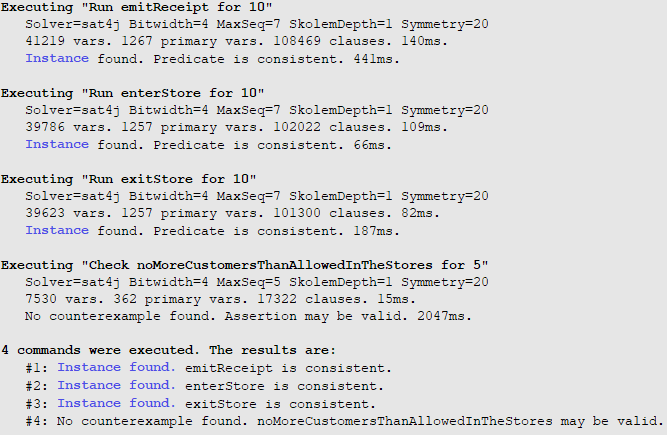
\includegraphics[width=\textwidth]{alloy_exec.png}
  \caption{Results of the execution of the Alloy predicates and assertions checks}
\end{figure}

\subsection{Resulting worlds}

\begin{figure}[H]
  \centering
  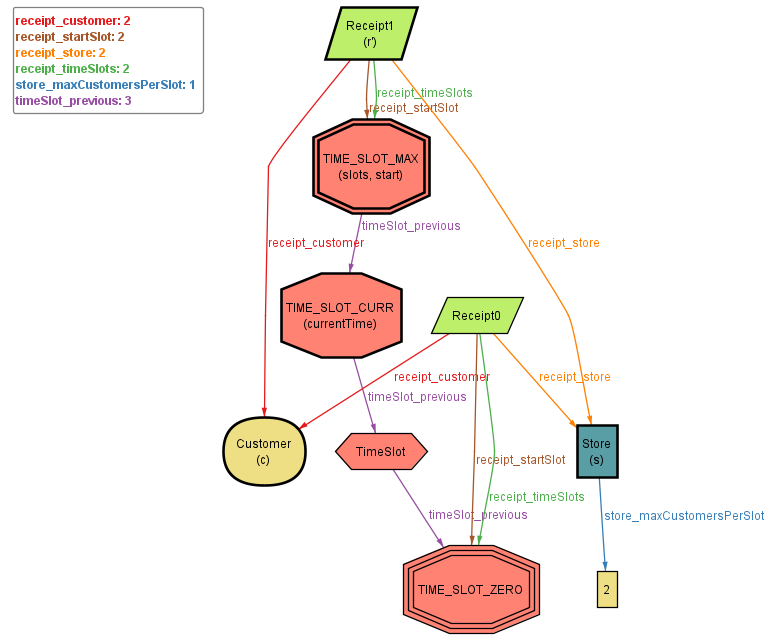
\includegraphics[width=\textwidth]{alloy_emitreceipt.png}
  \caption{One of the worlds generated by the emitReceipt predicate}
\end{figure}

\begin{figure}[H]
  \centering
  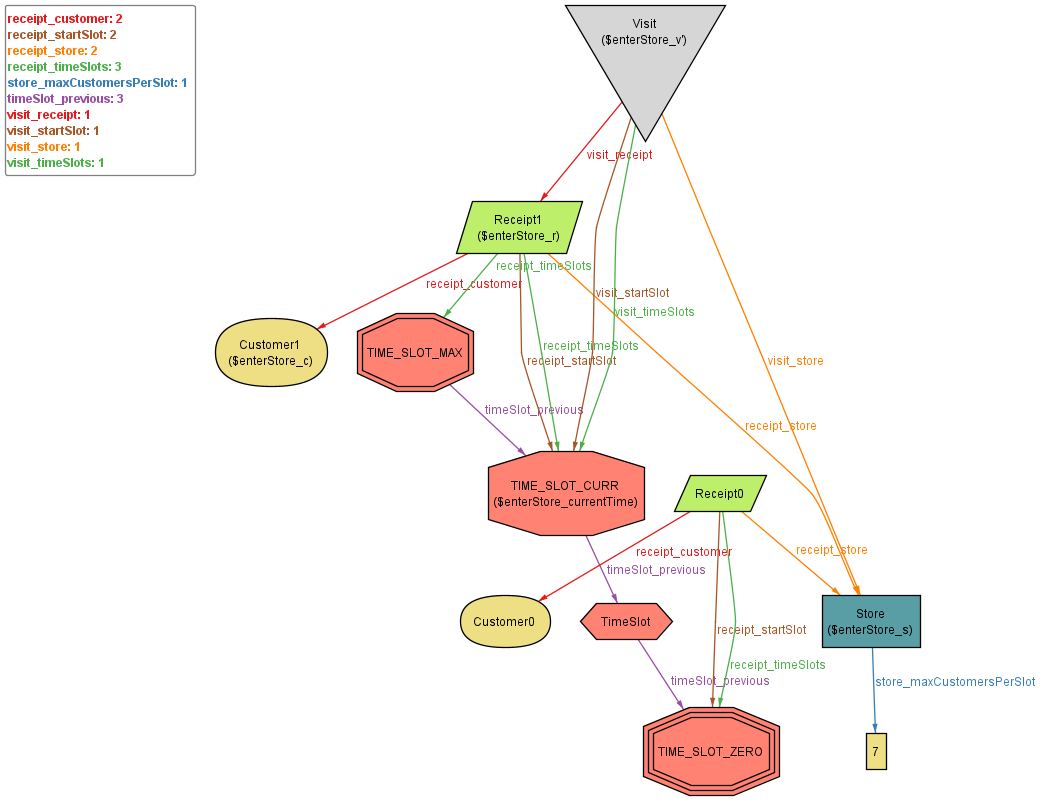
\includegraphics[width=\textwidth]{alloy_enterstore.png}
  \caption{One of the worlds generated by the enterStore predicate}
\end{figure}

\begin{figure}[H]
  \centering
  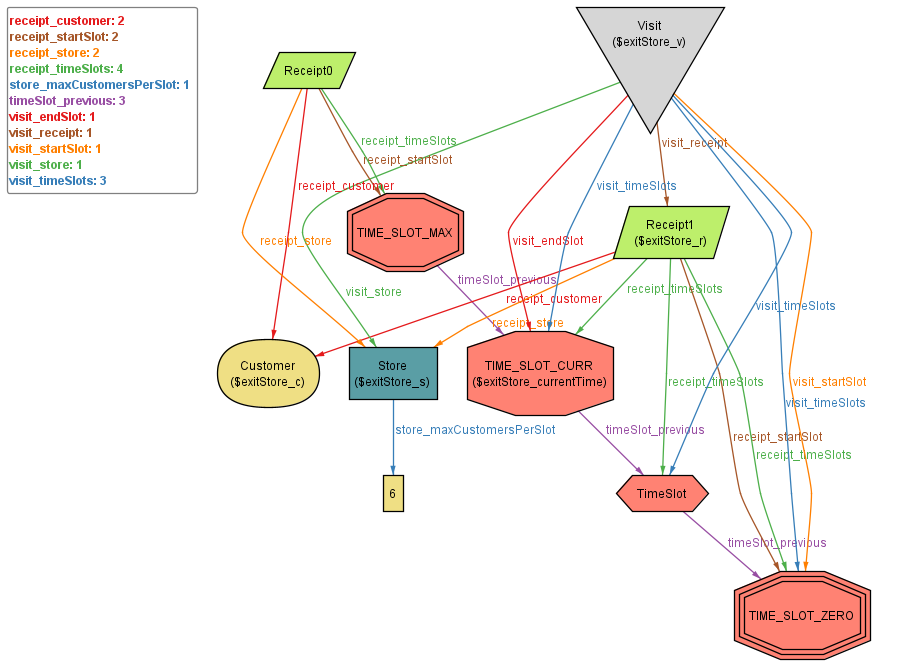
\includegraphics[width=\textwidth]{alloy_exitstore.png}
  \caption{One of the worlds generated by the exitStore predicate}
\end{figure}


\end{document}
